\documentclass[12pt,final,fleqn]{article}

% basic packages
\usepackage[margin=1in] { geometry }
\usepackage{amssymb,amsmath, bm}
\usepackage{verbatim}
\usepackage[latin1]{inputenc}
%\usepackage[OT1]{fontenc}
\usepackage{setspace}
\usepackage{enumitem}
\usepackage{url}
\usepackage[font={bf}]{caption}
\usepackage{float}
%\usepackage{pgfplots}
%\usepackage[font={bf}]{caption}
\usepackage{setspace}
\usepackage{latexsym}
%\usepackage{euscript}
\usepackage{graphicx}
\usepackage{marvosym}
\usepackage{amsmath} 
\usepackage{authblk}
\usepackage{xcolor}
%\usepackage[varg]{txfonts}  Older version of ``g'' in math.

% bibliography packages
\usepackage[natbibapa]{apacite}
\bibliographystyle{apacite}
\bibpunct{(}{)}{;}{a}{}{,}
\renewcommand{\bibname}{References}

% hyperref options
\usepackage{color}
\usepackage{hyperref}
\usepackage{xcolor}
\hypersetup{
    colorlinks,
    linkcolor={blue!50!black},
    citecolor={blue!50!black},
    urlcolor={blue!80!black}
}
\newcommand*{\Appendixautorefname}{Appendix}
\renewcommand*{\sectionautorefname}{Section}
\renewcommand*{\subsectionautorefname}{Section}
\newcommand{\aref}[1]{\hyperref[#1]{Appendix~\ref{#1}}}

% packages for tables
\usepackage{longtable}
\usepackage{booktabs, threeparttable}
\usepackage{threeparttablex}
%\usepackage{tabularx}
% dcolumn package
\usepackage{dcolumn}
\newcolumntype{.}{D{.}{.}{-1}}
\newcolumntype{d}[1]{D{.}{.}{#1}}
\captionsetup{belowskip=10pt,aboveskip=-5pt}
\usepackage{multirow}
% rotating package
\usepackage[figuresright]{rotating}
\usepackage{pdflscape}
\usepackage{subcaption}

% packages for figures
\usepackage{grffile}
\usepackage{afterpage}
\usepackage{float}
\usepackage[section]{placeins}


% theorem package
\usepackage{theorem}
\theoremstyle{plain}
\theoremheaderfont{\scshape}
\newtheorem{hyp}{Hypothesis}
\newtheorem{theorem}{Theorem}
\newtheorem{algorithm}{Algorithm}
\newtheorem{assumption}{Assumption}
\newtheorem{lemma}{Lemma}
\newtheorem{proposition}{Proposition}
\newtheorem{remark}{Remark}
\newcommand{\qed}{\hfill \ensuremath{\Box}}
\newcommand\indep{\protect\mathpalette{\protect\independenT}{\perp}}
\DeclareMathOperator{\sgn}{sgn}
\DeclareMathOperator{\tr}{tr}
\DeclareMathOperator{\argmin}{arg\min}
\DeclareMathOperator{\argmax}{arg\max}
\def\independenT#1#2{\mathrel{\rlap{$#1#2$}\mkern2mu{#1#2}}}
\providecommand{\norm}[1]{\lVert#1\rVert}
\renewcommand\r{\right}
\renewcommand\l{\left}
\newcommand\E{\mathbb{E}}
\newcommand\dist{\buildrel\rm d\over\sim}
\newcommand\iid{\stackrel{\rm i.i.d.}{\sim}}
\newcommand\ind{\stackrel{\rm indep.}{\sim}}
\newcommand\cov{{\rm Cov}}
\newcommand\var{{\rm Var}}
\newcommand\SD{{\rm SD}}
\newcommand\bone{\mathbf{1}}
\newcommand\bzero{\mathbf{0}}

% dotted lines in tables
%\usepackage{arydshln}

\usepackage{pdflscape}

% spacing between sections and subsections
\usepackage[compact]{titlesec}

% times new roman
%\usepackage{times}

% appendix settings
\usepackage[toc,page,header]{appendix}
\renewcommand{\appendixpagename}{\centering Appendices}
\usepackage{chngcntr}
\usepackage{etoolbox}
\usepackage{lipsum}


% file paths and definitions
\makeatletter
\newcommand*\ExpandableInput[1]{\@@input#1 }
\makeatother

\setlength{\mathindent}{1cm}
\allowdisplaybreaks[4]
\doublespacing
%\special{pdf: pagesize width 8.5truein height 11.0truein}

\titleformat{\subsection}
  {\itshape\large}{\thesubsection}{1em}{}

\setcounter{tocdepth}{1}

%--------------------------------------------------------------------------------------
% BEGIN DOCUMENT
%--------------------------------------------------------------------------------------

\begin{document}
\singlespace
\title{\textbf{Ballot initiatives and information processing, an experimental approach \\
(Pre-Analysis Plan)}\vspace{-1ex}\thanks{}}
% Direct democracy and special interest capture: experimental evidence from California
\author{Ang�le Delevoye\thanks{PhD Student in the Department of Political Science, Yale University. angele.delevoye@yale.edu}\vspace{-1ex}}
\author{Trevor Incerti\thanks{PhD Student in the Department of Political Science, Yale University. trevor.incerti@yale.edu}\vspace{-1ex}}
\affil{\textit{}\vspace{-2.5ex}}
\date{\today}
\maketitle

\begin{abstract}
\noindent
\vspace{10cm}
\end{abstract}

\pagebreak

\doublespace


\section{Introduction} \label{sec:Introduction}

One of the most direct ways in which citizens can produce policy is through pure democratic channels such as citizens initiatives, popular consultation, and ballot initiatives. Ballot initiatives have been hailed as an efficient direct democracy mechanism, providing citizens with a much-needed voice in policy making and politics. Defenders of ballot initiatives claim that they provide a way for citizens to voice their opinions and produce policies with less interference from parties and special interests [CITE]. Others caution against the excesses of direct democracy and claim that special interest capture also operates in this system [CITE]. Doubts about voters' competency are also central to whether ballot initiatives lead to adoption of good policies [CITE]. The need for technical knowledge may be larger on a ballot initiative than in a traditional partisan election as fewer heuristic cues are available. 

We therefore seek to determine how voters use information when asked to vote directly on a supposedly non-partisan, technical policy proposal placed on a ballot initiative. Are voters able to distinguish between the different levels of information quality and bias that stem from varying sources of information? Relatedly, do ballot initiatives actually lead to less interference from parties and special interests, or are voters equally swayed by special interests cues and objective policy research? 

We propose a field experiment examining voting outcomes on citizen initiated ballot propositions following randomized treatment of proposition endorsement or opposition by special interest groups and and policy experts during the 2020 California state elections. We seek to test whether citizens acting as policy makers give more credence to high quality policy research versus overtly partisan or biased information (i.e. special interests). In addition, we will replicate our field experiment with a survey experiment using identical subjects, treatments, and outcome measures.

The paper will contribute to the growing literature on the effect of campaign outreach on vote choice. Meta-analysis by \citet{kalla2018minimal} suggests that the effect of campaign contact and advertising on voting outcomes is close to zero in general elections. However, effects do seem to appear in non-partisan ballot measure campaigns, but few experiments exist on this topic. All ballot initiative experiments to date contact voters through a single advocacy group with a clear policy position. However, we know little about whether the quality and/or source of the information provided changes the efficiency of these messages. By contrast, our experimental design allows us to speak to the debate over whether direct democracy is actually more democratic than representative democracy, or if it suffers from the same elite manipulation might operate in both domains.
 
 A growing literature also suggests that survey experimental results often do not replicate in the field. For example, the zero effect of campaign contact in \citet{kalla2018minimal} does not replicate in survey experiments, and a recent meta analysis of the effects of providing voters with information about the corrupt actions of politicians shows an approximately zero effect in field experiments versus large negative effects in survey environments \citep{incerti2019corruption}. By contrast, we hypothesize that survey experiments should better approximate the context of ballot initiatives as: (1) the vote choices are real ballot propositions rather than hypothetical candidates, and (2) partisan cues are less prevalent in (technical) ballot proposals. Whether our hypothesis is correct or incorrect, we will contribute to the growing understanding of the contexts and questions in which survey experiments replicate or do not replicate in the real world.


\section{Theory} \label{sec:Theory}

\subsection{Science, research and democracy}  \label{sec: democracy}

This project speaks to broader theoretical questions on the functioning of our current democracies, and in particular the potential gaps between reality and the ideals of deliberative democracies. We hope therefore hope to contribute to ongoing discussions within philosophy of science, such as perceptions of research methods and consumption of scientific evidence outside of the academy. \\

[Tensions and relationships between science and democracy]

\subsection{Ballot initiatives and direct democracy}

Direct democracy at the US state-level is extremely prevalent yet understudied. 31 of 50 states permit referendums of some kind, and 24 permit citizen initiatives \citep{leduc2003politics}. Of these 24 states, California engages in more individual exercises of direct democracy than any other. Over the past two decades California has voted on X ballot initiatives at the statewide level [compare to other states], and the number of ballot initiatives per election has increased rapidly over the same period.

Some scholars view this growth of direct democracy as a positive extension of democratic values [CITE AND ADD MORE- SEE LEDUC, HELENE?].

Others contend that the initiative process in the United States has been captured by special interest groups, directly undermining the increased power ballot initiatives are designed to deliver to citizens [CITE - SEE LEDUC]. This implies that the outcomes of direct democracy are no more democratic than representative democracy, as the same elite manipulation that might operate in both domains. For example, the California initiative process has fostered the development of firms that collect signatures to meet required thresholds, and these firms are typically employed by special interest groups \citep{leduc2003politics}. Our research design allows us to evaluate the special interest capture theory by comparing the efficacy of special interest messages to those of independent policy analysts.

Ballot initiatives have also been identified as a source of major policy blunders. One of the most notorious of these blunders is California's Proposition 13 of 1978, which capped annual increases of real property taxes to 2 percent per year and prohibited governments from increasing property taxes without a further referendum. Proposition 13 has been blamed for underfunding of California public schools, contributing to California's housing crisis, and perpetuating income inequality in the state [CITE]. Proposition 13 was not without its critics at the time of passage, with critics contending that ``Proposition 13 raises serious questions about the feasibility of participatory democracy in a policy area which commonly has been dominated by experts'' \citep{mccaffery1978participatory}. In this context, our experimental design allows us to test whether voters are receptive to expert policy analysis warning of negative consequences of ballot referendum policies. 

In line with the partisan and special interest capture theories, as well as evidence that ballot initiatives often lead to policy blunders, our primary hypothesis is that \textit{voters will be equally swayed by information from special interest groups and policy researchers.} More formally, we expect the absolute value of special interest and policy research treatment effects to be statistically indistinguishable from one another.


%\citet{rosenbluth2018responsible} argue that decentralization of power to the grass roots level has worsened the quality of policy outputs and decision making in the United States by weakening parties.

\subsection{Current experimental evidence}  \label{sec: contact experiments}

A growing body of literature contends that information provision is relatively unsuccessful at changing voting outcomes. The primary conclusion of the Metaketa 1 project---which sought to determine if politicians were rewarded for positive information and punished for negative information---was that ``the overall effect of information [provision] across all studies is quite precisely estimated---and not statistically distinguishable from zero'' \citep{dunning2018metaketa}. \citet{incerti2019corruption} draws a similar conclusion in a meta-analysis of corruption information field experiments, finding no voter punishment of allegedly corrupt politicians across field experiments. In the US context, a meta-analysis by \citet{kalla2018minimal} suggests that the effect of campaign contact and advertising on voting outcomes is close to zero in general elections.

However, \citet{kalla2018minimal} find suggestive evidence that campaign contact produces positive effects on vote choice in ballot measure campaigns (see \autoref{fig: kb_meta}). While their meta-analysis includes 23 ballot initiative experiments, these experiments stem from 5 total projects \citep{arceneaux2005using, arceneaux2010comparing, rogers2015ballot}. All of these projects use advocacy groups to contact voters with a pro-initiative message via canvassing, phone, or mail. The existence of positive treatment effects in the ballot initiative environment begs the question of what kinds of informational campaigns are successful. Does high quality policy research persuade voters, or is special interest contact equally effective? 

%\citep{arceneaux2005using}: advocacy group, advocacy message, door to door canvassing, measured turnout and vote. Cluster design, precinct level.
%
%\citep{arceneaux2010comparing}: advocacy group, message tone (negative vs positive vs control), canvassing, measure turnout and vote. Two stage randomization approach, precinct level with clustering. 
%
%\citep{rogers2015ballot}: advocacy group, statewide mail program in Oregon, measure turnout and vote. 

\begin{figure}[h]
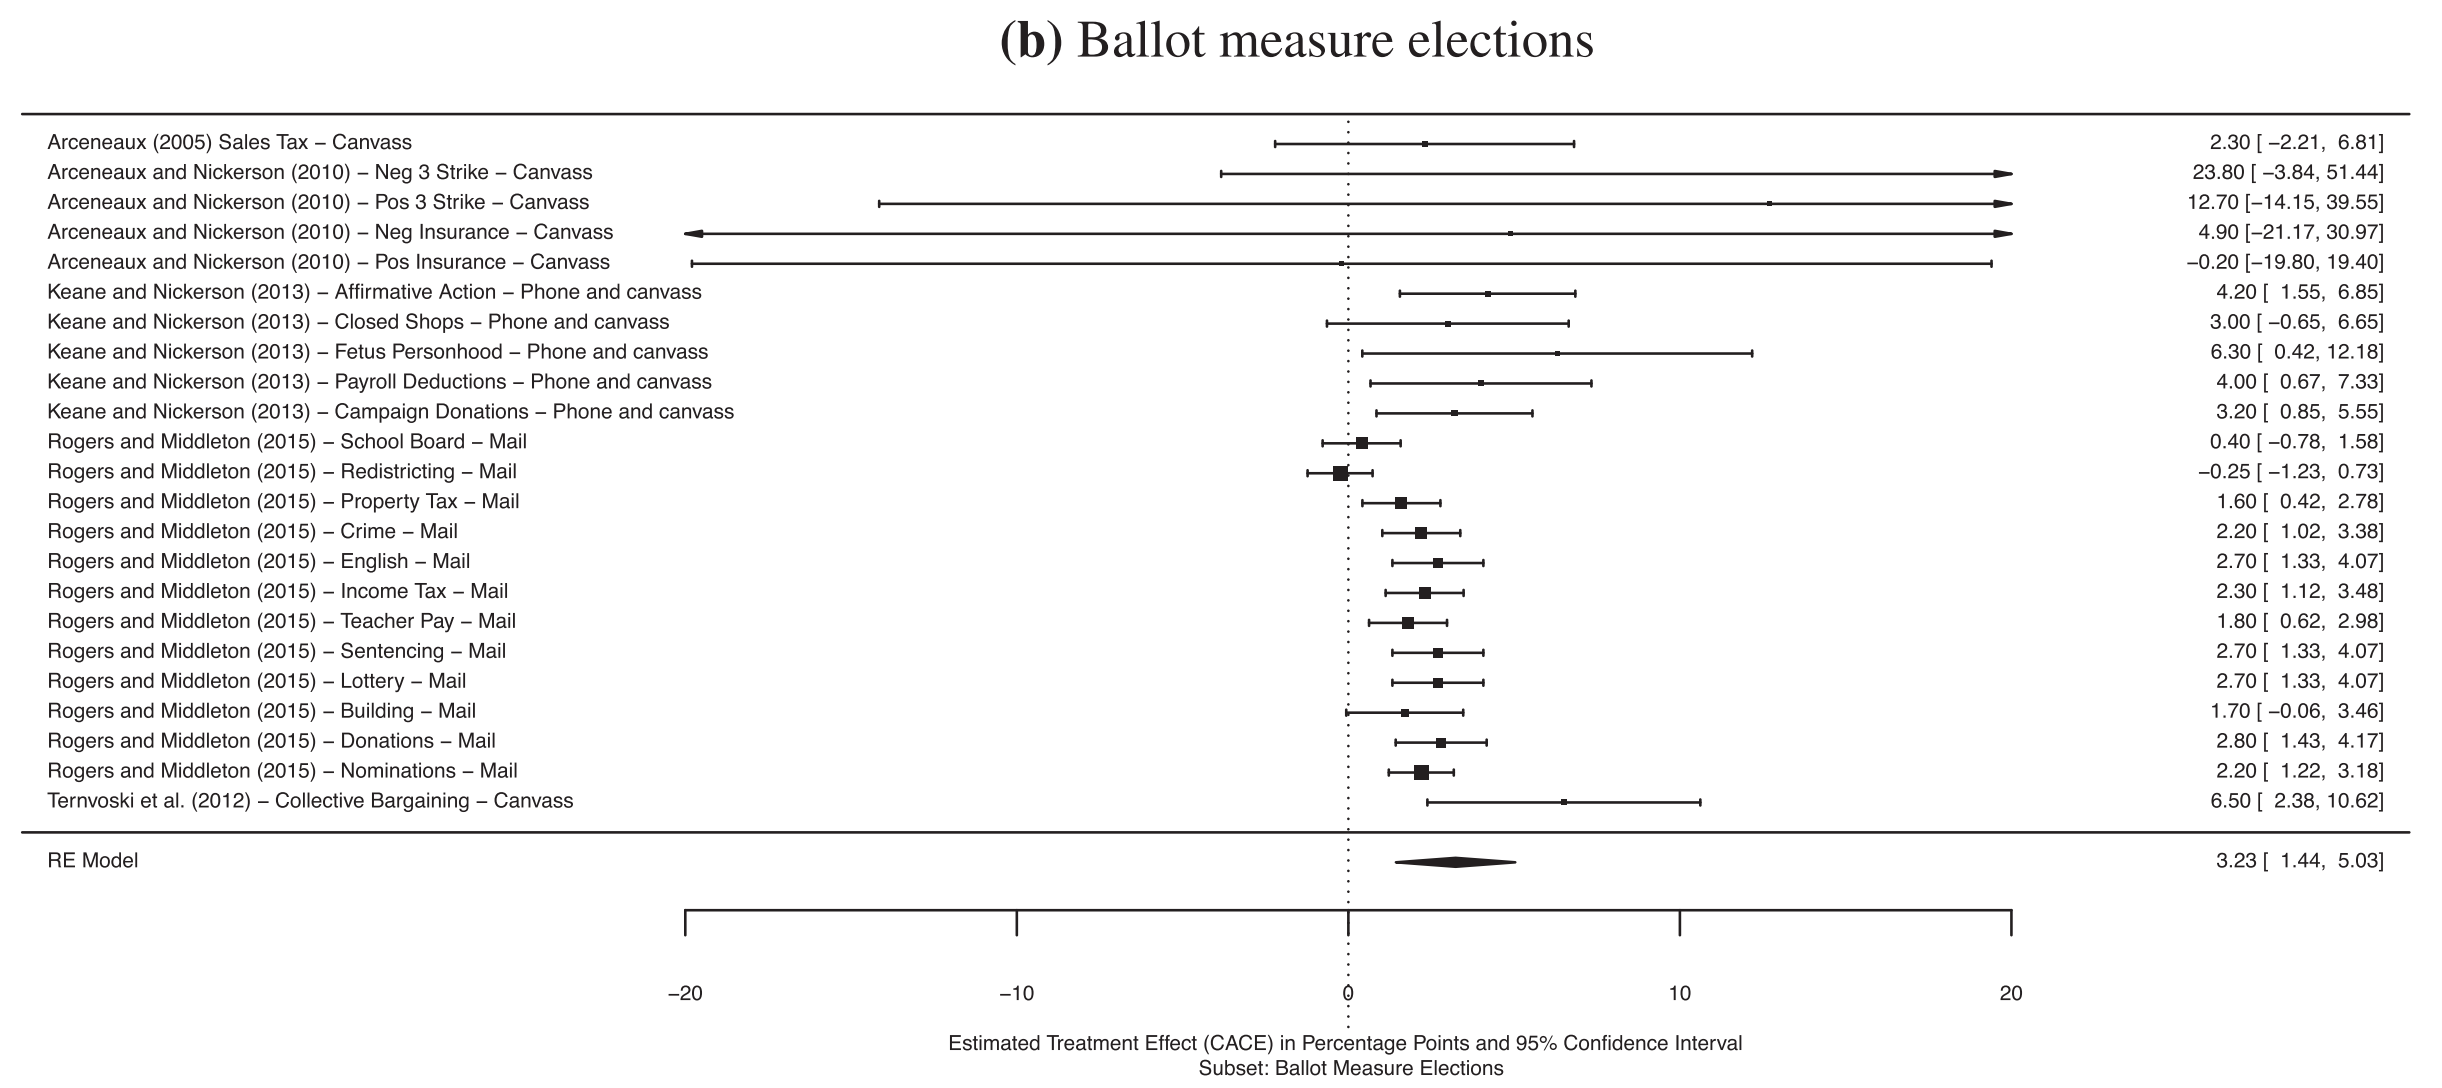
\includegraphics[scale=0.4]{meta_ballot}
\bigbreak
\caption{Meta Analysis of ballot initiative experiments from \citet{kalla2018minimal}}
\label{fig: kb_meta}
\end{figure}


\section{Field experiment} \label{sec:Design field}

\subsection{Treatment groups and randomization} \label{sec:Treatment}

We will provide voters with different randomized pieces of information encouraging either a ``Yes'' or ``No'' vote on a 2020 California ballot initiative. We will have three treatment groups in total: (1) placebo, (2) business/special interest group information, and (3) policy research information. Three treatment groups  allows us to have one null/zero treatment group (placebo), one positive treatment group, and one negative treatment, facilitating detection of differences between groups.

\subsection{Treatment details} \label{sec:Treatment}

This information provision could be done through mail (a postcard), canvassing, phone calls, text messaging, or emails. Postcards, text messaging, or email would provide allow for larger sample sizes than canvassing or phone calls. Extant literature on fliers as a persuasive source of information finds null treatment effects \citep{kalla2018minimal, incerti2019corruption}. However, it may be possible to improve upon previous field experiments by incorporating estimates of non-compliance rates into our experimental design, allowing us to estimate complier average causal effects (CACE) in addition to intent-to-treat (ITT) effects. For example, fliers could contain a link to a website with the informational treatment. We would then be able to use the percentage of individuals who received fliers that also accessed the website as an estimate of the proportion of compliers. This would allow us to measure the effect of \textit{reading} the informational treatment, rather than the effect of being assigned to the treatment group receiving the information. 

Canvassing would provide us with less power, less geographic reach, and would likely be costlier. However, direct contact has been shown to elicit larger treatment effects than other forms of communication \citep{kalla2018minimal}.

\subsection{Outcomes} \label{sec: Outcomes}

Our outcome measurement is percentage of ``Yes'' votes on the ballot initiative at the precinct or smaller level. This constitutes a theoretically direct outcome measurement, considering that we are interested in examining how susceptible voters in a direct democracy setting are to information campaigns by different groups. 

As our outcome is ``Yes" vote and we will provide one pro-initiative treatment and one negative anti-initiative treatment, we should illicit one positive treatment effect and one negative. If the absolute values of the treatment effects are the same, that supports the capture hypothesis (i.e. people weigh both sources of information equally). If the business treatment is smaller in absolute value, it disproves the capture hypothesis and suggests that people value research more than potentially biased information.

\subsection{Election cycle and choice of ballot measure} \label{sec:policy}

We seek to launch this experiment during the 2020 California statewide general election. An on-year election will give us access to a larger sample of likely voters in total, as well as a greater percentage of voters without strong priors on the specific proposal. Off-year voters tend to be more informed about specific ballot measures and therefore have stronger priors and are less susceptible to informational campaigns. 

Our ideal ballot measure would involve a policy with a scientific or policy research consensus on its overall merit or demerit. This would likely represent a technical subject on which people have relatively weak priors. For example: Health care, housing, etc. A list of 2020 California ballot measures or those approved by yet to meet the minimum signature threshold eligible or requiring additional is provided in \autoref{tab: initiatives}.

\begin{table}[!htbp] \centering 
  \caption{Potential 2020 California ballot initiatives as of June 2019}
  \label{tab: initiatives} 
  \small
\begin{tabular}{@{\extracolsep{0pt}} cccccccc} 
\\[-1.8ex]\hline 
\hline \\[-1.8ex] 
 Initiative & Topic & Endorsement & Approved & Ideal \\ 
\hline \\[-1.8ex] 
Jury trials for child custody & Legal & NA & Yes & No \\
Rental Affordability Act & Housing & NA & No & Maybe \\
Risk-based bail & Criminality & NA & No & No \\
Number of candidates in general elections & Politics & NA & No & No \\
GMO ban (SI) & Health & NA & No & Maybe \\
Fluoride ban (SI) & Health & NA & No & Maybe \\
Remove school vaccine requirement (SI) & Health & NA & No & Maybe \\
Supermajority for revenue measures & Politics & NA & No & No \\
Amend three strikes law & Criminality & NA & No & Maybe \\
Felony for some misdemeaners & Criminality & NA & No & Maybe \\
Confinement of farm animals & Agriculture & NA & No & No \\
Estate tax for college aid & Tax \& Education & NA & No & Maybe \\
No changes on approved bond spending & Politics & NA & No & Maybe \\
Elimination of Open Ended Alimony & Legal & NA & No & No \\
\hline \\[-1.8ex] 
\end{tabular} 
\end{table} 
\FloatBarrier

\subsection{Estimation of treatment effects} \label{sec:treatment_effects}

We intend to use block random assignment in order to increase the precision of our treatment effect estimates as well as to facilitate (preregistered) estimation of heterogenous treatment effects. Treatment effect estimates will therefore be calculated as the difference-in-means of the response rate from subjects in each of treatment groups and the response rate from subjects in the control group in each block, weighted by the number of subjects in each block relative to the total number of subjects. More formally, average treatment effects will be estimated as:

\begin{center}
$ATE = \sum_{j = 1}^{J} \frac{N_j}{N}ATE_j$
\end{center}

\noindent
where $J$ is the number of blocks, blocks are indexed by $j$, and $\frac{N_j}{N}$ represents the share of subjects who belong to block $j$. In practice, these differences-in-means will be calculated using a weighted least squares regression of response rate on treatment assignment, with weights corresponding to the inverse probability of treatment for each unit (IPW). All p-values will be calculated using randomization inference.

\subsection{Heterogenous treatment effects} \label{sec: hte}

In addition, we will test for heterogenous treatment by party affiliation and educational attainment. Our test will take the form of regressing our outcome variable on treatments conditional upon the data representing the covariate of interest. In other words, we will split our sample by subject attributes (party and educational attainment), then estimate conditional average treatment effects (CATEs) separately for each of these attributes. For example, to test for heterogenous effects by party, we will regress outcomes on treatments for all voters in each party. Following estimation of CATEs, we will use randomization inference to test the null hypothesis that CATEs in both groups (e.g. Democrat and Republican) equal to the ATE.

We recognize that the search for heterogenous treatment effects often suffers from the multiple comparisons problem. In a dataset with a large number of covariates, if a large enough number of subgroups is examined, it is highly likely that statistically significant interaction effects will emerge merely by chance. In other words, the more significance tests are performed, the higher the likelihood of falsely rejecting the null hypothesis at least once. We minimize this risk be preregistering our heterogenous effects of interests, as well as by performing multiple comparisons corrections using Bonferroni, Holm-Bonferroni, and Benjamin-Hochburg adjustment procedures.

\subsection{Power analysis} \label{sec: power}


\section{Survey experiment} \label{sec:Design survey}

\subsection{Why do a survey experiment?} \label{sec: questions}

 A growing literature suggests that survey experimental results often do not replicate in the field. By contrast, we hypothesize that survey experiments should better approximate the context of ballot initiatives as: (1) the vote choices are real ballot propositions rather than hypothetical candidates, and (2) partisan cues are less prevalent in (technical) ballot proposals. The ballot initiative setting would allow us to design the survey so that it exactly replicates the field setting, with the only differences being hypothetical vote choice versus actual.
 
Whether our hypothesis is correct or incorrect, we will contribute to the growing understanding of the contexts and questions in which survey experiments replicate or do not replicate in the real world. If our hypothesis is correct, we can open the door for more survey experiments with more varied and ambitious treatments. If our hypothesis is incorrect, we show that survey experiments do not replicate even in a context where they closely approximate the field environment.

\subsection{Design} \label{sec: questions}

The ballot initiative setting would allow us to create a survey experiment in which the subjects, treatment, and outcome variable are identical to those in the field setting. In other words, we could sample from the same population, use the same informational treatments that would be sent to voters in the field setting, and measure the same outcome---vote choice---with the exception that the outcome is real in the field setting and hypothetical in the survey setting. 

\section{Natural experiment} \label{sec:natural}

The idea would be to use a real-life variation of information supply. Ex.: data on billboards, with their contents and where exactly they were put on, or a report sent to some precinct but not other. Info provision will probably not be random, so we would need to do a diff and diff (precinct with billboard ? precinct without billboard, but which other difference? Vote on another measure, vote in previous elections, opinion polls on the measure before billboards went up, early voting)? \\

[SIGNATURE REQUIREMENT THRESHOLD AS DISCONTINUITY: LET'S THINK ABOUT THIS. MAYBE TALK TO FREDRIK.]

\section{Conclusion} \label{sec:Conclusion}

Our next steps on this project include finalization of some of the research design decisions that remain open (i.e. choice of ballot initiative, location and creation of informational messages, possible partnership with organizations). We hope to finalize these details over the summer and to preregister a final Pre-Analysis-Plan with EGAP by the end of 2019. We would then conduct the experiment immediately prior to the 2020 California state general elections.



\clearpage
\pagebreak
\bibliography{bibliography}

\pagebreak

\appendix
\setcounter{table}{0}
\setcounter{figure}{0}
\renewcommand\thetable{\Alph{section}.\arabic{table}}
\renewcommand\thefigure{\Alph{section}.\arabic{figure}}
\section{Appendix} \label{Appendix}





\end{document} 